\section{Detectare bandă}
\subsection{Noțiuni introductive}
O primă componentă a aplicației de față este ceea care se ocupă de detecția benzi curente de circulație. Scopul acesteia este de a identifica marcajele, atât cele continue, cât și cele discontinue, pe baza cărora va indica banda curentă de circulație a mașinii.

\subsection{Algoritm detecție bandă}
\subsubsection{Etapa 1: Extragere regiune interes}

Această etapă are rolul de a elimina din imagine zonele redundante detecției. Atât în situația de față, cât și ulterior în cazul detecției de mașini, ne putem focusa pe o anumită zonă din cadrul frame-ului pentru a detecta banda curentă de circulație și ulterior mașina de pe aceasta. Această zonă este direct determinată de cameră, rezoluție acesteia, amplasarea camerei pe mașină, iar în funcție de toți acești factori se va crea un fișier de configurație specific montajului respectiv cu parametri necesari extragerii zonei de interes.

În figura 3.1 putem observa un exemple concrete.
\begin{figure}[!h]
	\centering
	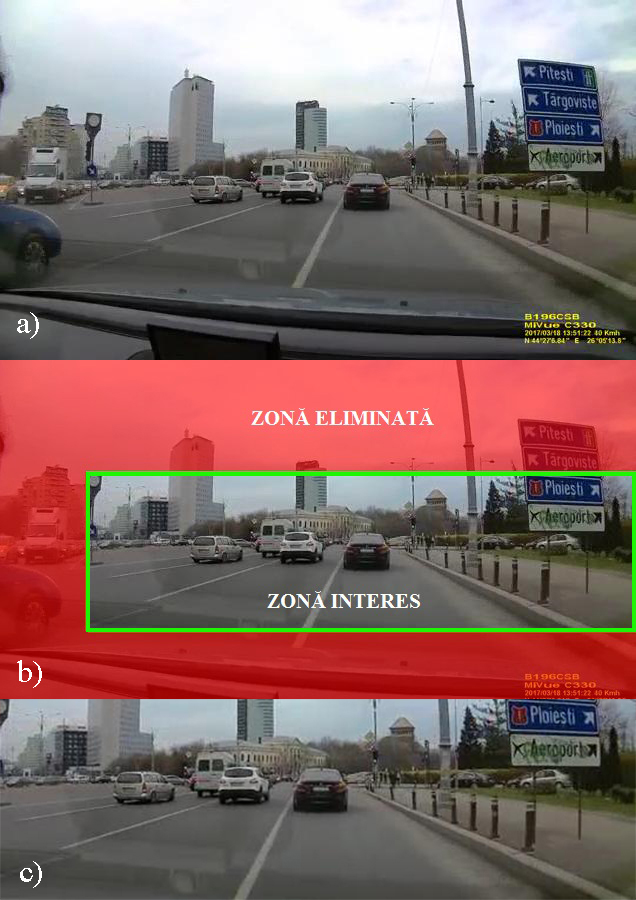
\includegraphics[max width=15cm,max height=15cm,keepaspectratio]{img_3_1}
	\caption[Zonă interes imagine]{a) Imaginea inițială b) Separația zonei de interes față de cea redundantă c) Imaginea de interes rezultată.}
\end{figure}

\subsubsection{Etapa 2: Obținere imagine IPM}

Următoare etapă în procesul de detecție a benzii curente de circulație este cea în care vom schimba perspectiva de vizualizare a zonei de interes. Prin intermediul unui fișier de configurare se vor da parametri ce vor fi folosiți ulterior în funcțiea de obținere IPM. Fie A, B, C și D punctele extreme ale imaginii. Vom redefini punctele B și C conform figurii 3.2. Cei doi vectori de puncte îi pasăm funcției $cv.getPerspectiveTransform$ din biblioteca OpenCV spre a obține matrice $M$ de trecere din perspectiva a), conform figurii 3.2, în perspectiva b). Matricea $M$ este folosită în continuare cu funcția $cv.warpPerspective$ pentru pentru a obține imaginea în planul IPM.
\begin{figure}[!h]
	\centering
	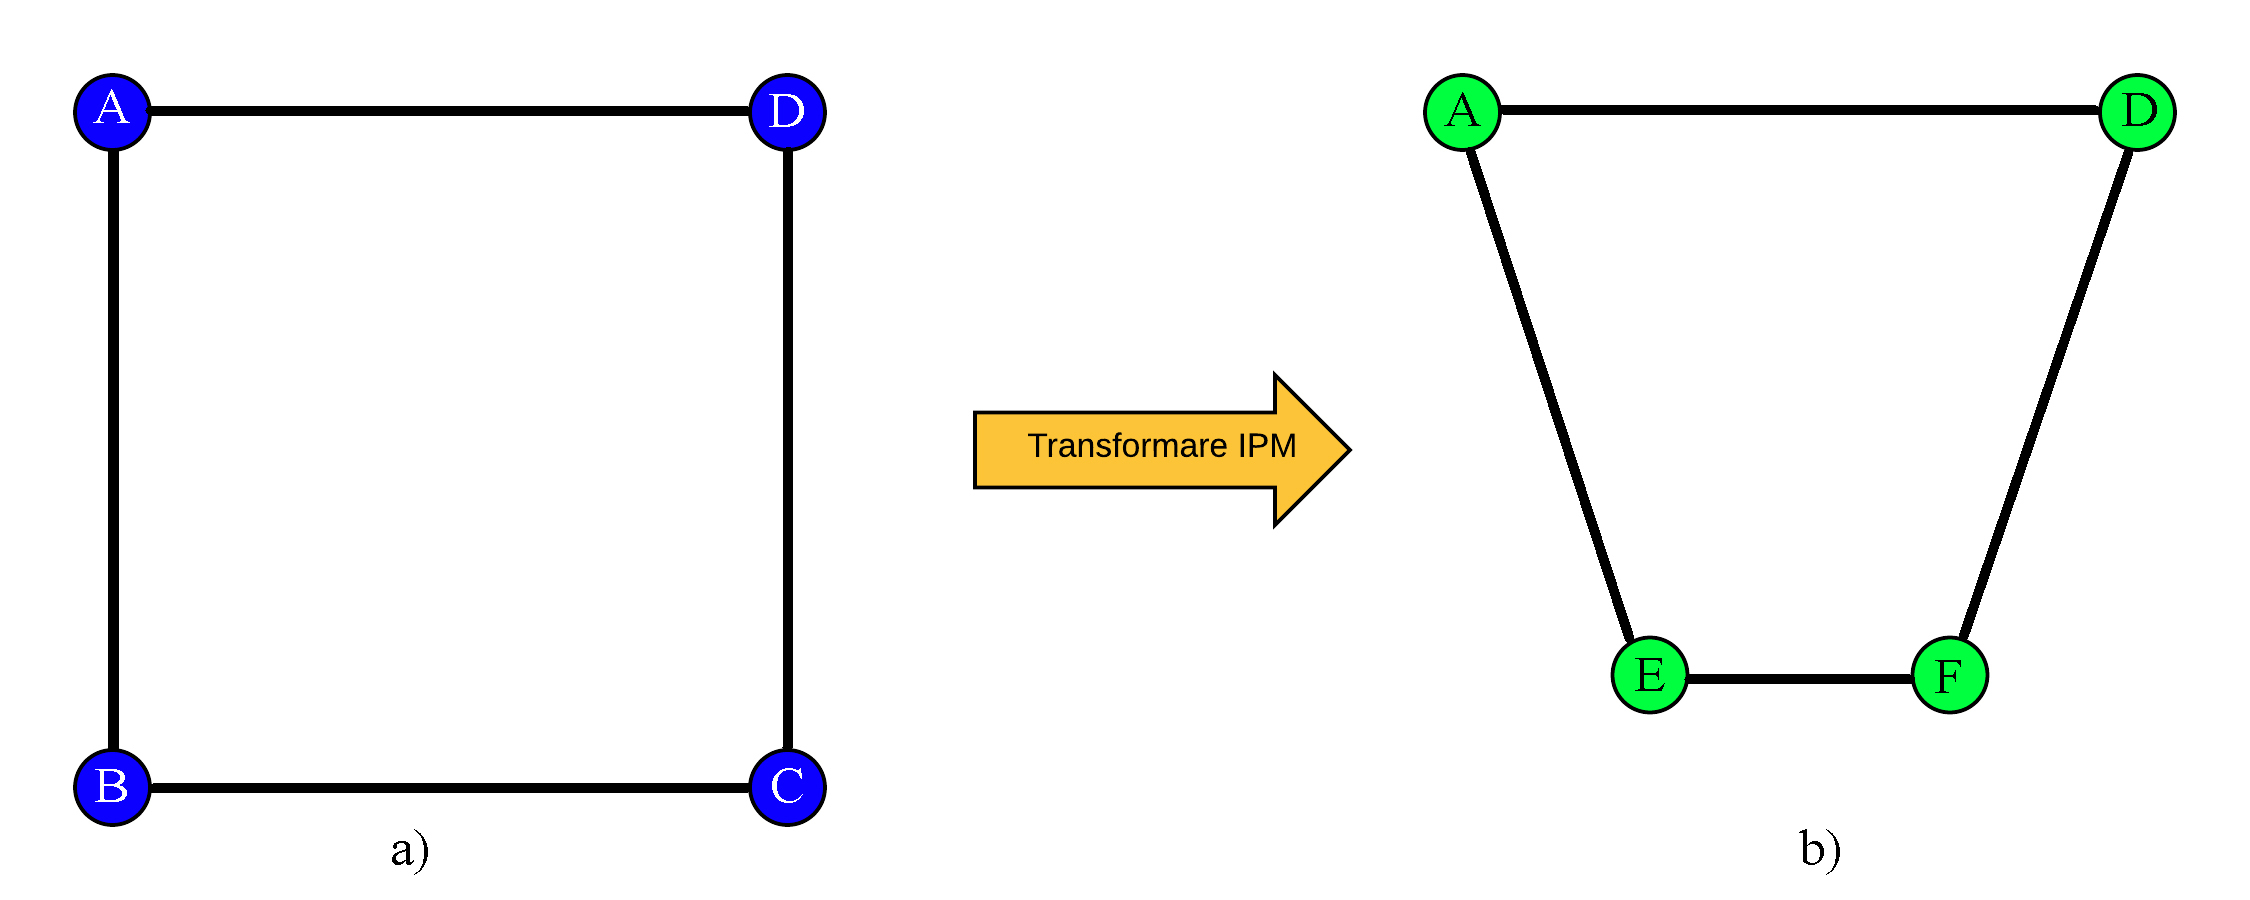
\includegraphics[max width=15cm,max height=15cm,keepaspectratio]{img_3_2}
	\caption[Transformare IPM]{a) Cadrul imaginii inițiale b) Cadrul imaginii IPM. Punctele B și C, din cadrul imaginii inițiale, sunt redefinite în punctele E și F.}
\end{figure}

În figura 3.3 este prezentat un exemplu practic.
\begin{figure}[!h]
	\centering
	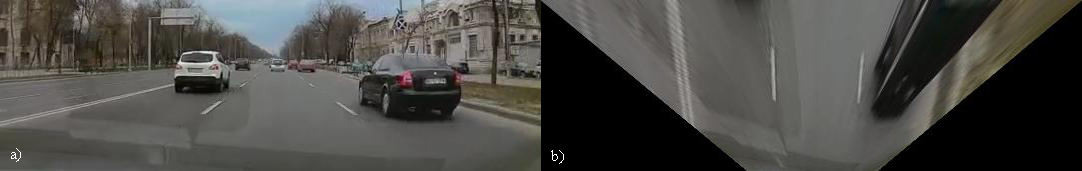
\includegraphics[max width=15cm,max height=15cm,keepaspectratio]{img_3_3}
	\caption[Transformare IPM în practică]{a) Imagine zonă interes b) Imaginea IPM asociată zonei de interes.}
\end{figure}


\subsubsection{Etapa 3: Filtrarea imaginii IPM}

Filtrarea imaginii IPM are rolul de a păstra în imagine doar zonele cele mai plauzibile de a fi marcaje delimitatorii de bandă și eliminarea celulalt conținut. Noua imagine, imagine, va fi o imagine binară de alb și negru. Pentru filtrare se folosește filtrul Gaussian orizontal
$ FG = 
\begin{bmatrix}
	0 & 0 & 0 \\
	0 & 1 & -1 \\
	0 & 0 & 0 \\
\end{bmatrix}
$
\begin{figure}[!h]
	\centering
	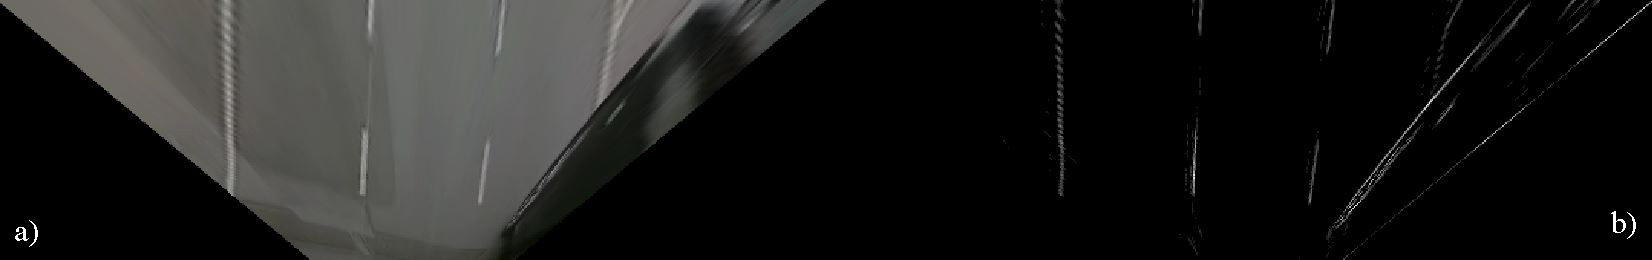
\includegraphics[max width=15cm,max height=15cm,keepaspectratio]{img_3_4}
	\caption[Imagine IPM filtrată]{a) Imaginea IPM b) Imaginea IPM filtrată.}
\end{figure}

\section{Detectare mașină}
\subsection{Noțiuni introductive}
\subsection{Algoritm detecție mașină}

\section{Determinare distanță}
\subsection{Noțiuni introductive}
\subsection{Algoritm determinare distanță}

\section{Determinare viteză relativă}
\subsection{Noțiuni introductive}
\subsection{Algoritm determinare viteză relativă}